% !TEX TS-program = pdflatex
% !TEX encoding = UTF-8 Unicode

% This is a simple template for a LaTeX document using the "article" class.
% See "book", "report", "letter" for other types of document.

\documentclass[11pt]{article} % use larger type; default would be 10pt

\usepackage[utf8]{inputenc} % set input encoding (not needed with XeLaTeX)

%%% Examples of Article customizations
% These packages are optional, depending whether you want the features they provide.
% See the LaTeX Companion or other references for full information.

%%% PAGE DIMENSIONS
\usepackage{geometry} % to change the page dimensions
\geometry{a4paper} % or letterpaper (US) or a5paper or....
% \geometry{margin=2in} % for example, change the margins to 2 inches all round
% \geometry{landscape} % set up the page for landscape
%   read geometry.pdf for detailed page layout information

\usepackage{graphicx} % support the \includegraphics command and options

% \usepackage[parfill]{parskip} % Activate to begin paragraphs with an empty line rather than an indent

%%% PACKAGES
\usepackage{booktabs} % for much better looking tables
\usepackage{array} % for better arrays (eg matrices) in maths
\usepackage{paralist} % very flexible & customisable lists (eg. enumerate/itemize, etc.)
\usepackage{verbatim} % adds environment for commenting out blocks of text & for better verbatim
\usepackage{subfig} % make it possible to include more than one captioned figure/table in a single float
% These packages are all incorporated in the memoir class to one degree or another...

%%% HEADERS & FOOTERS
\usepackage{fancyhdr} % This should be set AFTER setting up the page geometry
\pagestyle{fancy} % options: empty , plain , fancy
\renewcommand{\headrulewidth}{0pt} % customise the layout...
\lhead{}\chead{}\rhead{}
\lfoot{}\cfoot{\thepage}\rfoot{}

%%% SECTION TITLE APPEARANCE
\usepackage{sectsty}


\allsectionsfont{\sffamily\mdseries\upshape} % (See the fntguide.pdf for font help)
% (This matches ConTeXt defaults)

%%% ToC (table of contents) APPEARANCE
\usepackage[nottoc,notlof,notlot]{tocbibind} % Put the bibliography in the ToC
\usepackage[titles,subfigure]{tocloft} % Alter the style of the Table of Contents
\renewcommand{\cftsecfont}{\rmfamily\mdseries\upshape}
\renewcommand{\cftsecpagefont}{\rmfamily\mdseries\upshape} % No bold!

%%% END Article customizations


\usepackage[bulgarian]{babel}
\usepackage{physics}
\usepackage{amsmath}
\usepackage{centernot}
\usepackage{url}
\usepackage{graphicx}
\graphicspath{ {.} }
\usepackage{amsfonts}
\usepackage{xcolor}
\usepackage{enumitem}
\usepackage{systeme}
\usepackage{listings}
\usepackage[cache=false]{minted}
\usepackage{csquotes}
\setquotestyle{english}



%%% The "real" document content comes below...

\title{20. Проектиране и интегриране на софтуерни системи}
\author{Play4u}
%\date{} % Activate to display a given date or no date (if empty),
         % otherwise the current date is printed
         

\newcommand{\lrangle}[1]{\left\langle #1 \right\rangle}

\newcommand{\oversetModels}[1]{\overset{#1}{\models}}

\newcommand{\italicBold}[1]{\textbf{\emph{#1}}}

\newcommand{\definition}{\italicBold{Дефиниция: }}
\newcommand{\theorem}{\italicBold{Теорема: }}
\newcommand{\lemma}{\italicBold{Лема: }}
\newcommand{\proof}{\italicBold{Доказателство: }}
\newcommand{\statement}{\italicBold{Твърдение: }}
\newcommand{\source}{\italicBold{Източник: }}

\newcommand{\integral}[4]{\displaystyle \int_{#1}^{#2}#3\,#4}

\newcommand{\redText}[1]{\textcolor{red}{#1}}

\newcommand{\curlies}[1]{\{#1\}}
\newcommand{\overbar}[1]{\mkern 1.5mu\overline{\mkern-1.5mu#1\mkern-1.5mu}\mkern 1.5mu}


\newcommand{\enumNum}{\renewcommand{\theenumi}{\arabic{enumi}}}
\newcommand{\enumlet}{\renewcommand{\theenumi}{\alph{enumi}}} 

\begin{document}
\maketitle

\italicBold{Конспект: } Изложението на въпроса трябва да включва следните по-съществени елементи:

\enumNum
\begin{enumerate}[noitemsep]
	\item Характеристика на разпределените софтуерни системи - дефиниции, видове системи и тенденции
	\item Междупроцесна комуникация - отдалечено извикване, млултикаст
	\item Разпределени обекти и компоненти
	\item Уеб услуги - дефиниции, шаблони за комникация. Стандарти за уеб услуги - SOAP, UDDI, WSDL.\\\par
\end{enumerate}


\section{Характерстики}
\subsection{Дефниции}
Разпределена система е такава, чиито компоненти са разположени на различни, свързани чрез мрежа, компютри, които си комуникират и се координират чрез размяна на съобщения помежду си. - Wikipedia\\
Разпределената система представлява съвкупност от компютри, които изглеждат на потребителите си като една кохерентна система. - Таненбаум\\
Разпределената система е съвкупност от автономни хостове, които са свързани чрез компютърна мрежа. Всеки хост изпълнява компоненти и върху него работи разпределен middleware, който позволява компонентите да координират своите активности по такъв начин, че потребителите да възприемат системата като единично, интегрирано средство за работа. - Емерих\\\par

\italicBold{Middleware (Опционално: )}\\
С усложняването на софтуера се налага и по-голяма абстракция и все по-сложни примитиви за разработка. Така се преминава от операционни системи към мрежови операционни системи докато се стига до нуждата от нов абстрактен слой, който да предоставя основни услуги и който има за цел прозрачност на разпределеността на системата. Този слой се нарича middleware.\\
\definition Middleware е термин, който се отнася до множеството от софтуерни услуги, което се намира между приложението и операционната система и има за цел да улесни разработването на разпределени приложения чрез абстрахиране от сложеността и хетерогенността на намиращата се отдолу сред операционни системи, хардуерни платформи и комуникационни протоколи.\\\par

\subsection{Разпределени системи}
\begin{itemize}[noitemsep]
	\item \textbf{Client-Server: } В този тип системи клиентското приложение изисква някакъв ресурс, който сървъра предоставя. Един сървър може да обслужва множество клиенти едновременно, за разлика от клиента, който може да е в контакт само с един сървър. Обикновено и клиентът, и сървърът са в една и съща компютърна мрежа, затова се счита, че те са част от разпределените системи. 
	\item \textbf{Peer-to-Peer: } Тези системи са изградени от върхове(nodes) - компютри - които имат еднакъв статут при споделянето на данни помежду си. Всички задачи се разпределят равномерно сред върховете. Те взаимодействат един с друг, споделяйки ресурси. Това се случва с помощта на мрежата с която са свързани.  
	\item \textbf{Трислойни: } Информацията на клиента се съдържа в средния слой, вместо в клиентския слой, с цел улесняване на интеграцията на приложението. Този архитектурен модел се среща най-честно сред уеб приложенията.
	\item \textbf{N-слойни: } В най-общия случай се изплолзва , когато приложение или сървър трябва да препрати заявки към други бизнес услуги на същата мрежа. 
	\item \textbf{Push model: } Сървърът инициира диалога. \enquote{Push-ва} информация към клиента. Клиентът слуша за \enquote{push-ове} от сървъра. Пр.: WAP, SMS.
	\item \textbf{Multiple servers: } Услугите са предоставени от множество сървъри. Разделени на части или репликирани обекти, свързани с услугите. Репликацията предоставя: По-добър performance, наличност и устойчивост на грешки. Но за сметка на това изисква координация.
	\item \textbf{Прокси сървъри и кешове: } \textbf{Кеш}: място, което съдържа наскоро използвани данни. Подобрява Performence-a на много приложения многократно. Но изисква протоколи за проверка вярността на кеш-а. \textbf{Прокси сървър}: Споделен кеш с ресурси. Прави репликацията и разпространението на данни транспарантно. Най-често се използва за достъп до мрежата. За разлика от 3-слойната архитектура, прокситата само кешират данните - не оперират върху тях.
	\item \textbf{Мобилни агенти: } Работеща програма(код и дати?). Преминава от един компютър в мрежата до друг. Изпълнява някакви задачи от името на друг процес. Може да достъпва локалните ресурси на компютрите които посещава.
	\item \textbf{Network cоmputers/Тънки клиенти: } \textbf{Network computer: }Всички файлове се съдържат отдалечено. Колкото се може по-малко локален софтуев и хардуер. Всеки локален диск може да се използва като кеш. \textbf{Тънък клиент: } Поддържа базиран на прозорци UI на локалния компютър. Потребителят може да изпълнява приложения на отдалечения компютър, локално. Ниски разходи по хардуера, и няма нужда от много управление на клиента. Може да страда от мрежови и OS забавяния.
	\item \textbf{Мобилни устройства: } Хардуерни изчислителни компоненти. Могат да се придвижват между различни физически локации. Могат да се използват за внезапни изчисления и inter-operation?. Откриването на услуги от тях е много важно. \\\par
\end{itemize}

\subsection{Тенденции}
\source \path{https://www.quora.com/What-are-the-trends-in-distributed-systems}
\begin{itemize}[noitemsep]
	\item The emergence of pervasive networking technology
	\item The emergence of ubiquitous computing
	\item The increase in demand for multimedia services
	\item View of distributed systems as a utility
\end{itemize}

\section{Meждупроцесна комуникация}
Процесите си комуникират чрез размяна на съобщения. Операционните системи предоставят инструменти за контролиране на междупроцесната комуникация(IPC), като \textit{опашки със съобщения, смеафори и споделена памет}. Middleware-ът използва тези инструменти за да предостави, от своя страна, application programming interface(API), което позволява IPC- да бъде програмирана на по-високо ниво на абстракция. Разпределените системи изискват размяната между независими процеси да се случва чрез следните две важни операции: 
\begin{enumerate}[noitemsep]
	\item send(message)
	\item receive(message)\\\par
\end{enumerate} 

\textit{\textbf{Connection-oriented IPC: }} Нека p и q са процеси. Тогава те си комуникират като:
\begin{enumerate}[noitemsep]
	\item установяват комуникационна връзка помежду си(физическа сесия)
	\item Си предават съобщения чрез send/receive операции\\
\end{enumerate}
\begin{center}
	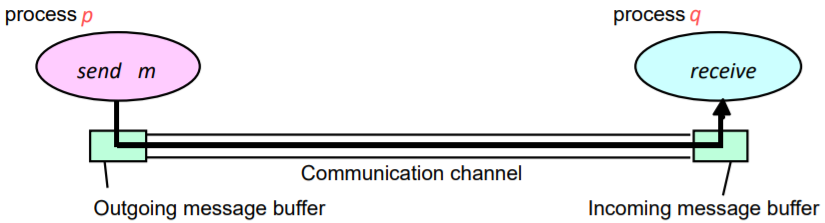
\includegraphics[scale=0.5]{ConnectionOrientedIPC.png} 
\end{center}
\newpage
\textit{\textbf{Message-oriented IPC: }}\\
\begin{center}
	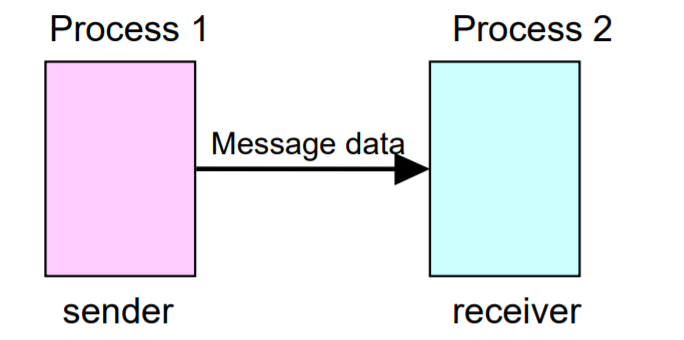
\includegraphics[scale=0.5]{MessageOrientedIPC.png} 
\end{center}

\subsection{Multicast}
В разпределените системи, два или повече процеса участват в един IPC протокол, избран от тях. Даден процес може да бъде sender в определен момент от времето и receiver в друг. Когато комуникацията е от един процес до един едиствен друг процес, тогава IPC се нарича \textbf{unicast}. Когато комуникацията е от един процес към \textit{група} процеси, тогава IPC се нарича \textbf{multicast}

\begin{center}
	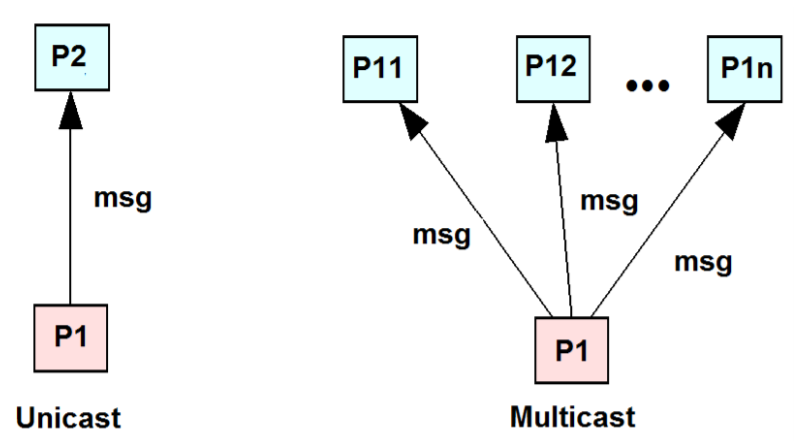
\includegraphics[scale=0.5]{UniMulticast.png}
\end{center} 
 
\textbf{Мултикаст операциите: } Изпълняват групови операции. Могат да използват транспортния протокол за да контролират пътя на комуникацията. Обикновено са базирани на broadcast моделите, за разлика от point-to-point връзките.\\\par
\textbf{Плюсове на мултикаст: } 
\begin{itemize}[noitemsep]
	\item Устойчивост на грешките, базирана на репликираните услуги: заявките се multicast-ват до множество сървъри и въпреки, че някои от тях може да не я изпълнят, стига един да я изпълни, клиента ще получи резултат.
	\item Динамично отркиване на услуги чрез сканиране и probing: Multicast-ваме за да открием кой има услугите, които търсим.
	\item По-добър performance чрез репликация на данните: multicast updates.
	\item Асинхронни нотификации за събития: пр. появата на нови артикули, услуги за реклама.
\end{itemize}
Устойчивост на грешки, базирано на репликирани услуги.\\\par 

\textbf{Имплементация на Multicast, използвайки UDP}\\
\enumNum
\begin{enumerate}[noitemsep]
	\item Установяваме мрежа от peer-и.
	\begin{itemize}[noitemsep]
		\item Изпозваме клас D адреси(първите 4 бита са \textbf{1110} в IPv4)
		\item Мултикаст алокацията на адреси може да постоянна или временна.
		\begin{itemize}[noitemsep]
			\item Без централен регистър
			\item time to live(TTL) ограничава броя прескачания(hops) и така ограничава дистанцията
			\item инструменти като \enquote{сесийна директория} могат да помогнат с управлението и намирането на multicast адреси. 
		\end{itemize}
	\end{itemize}
	\item Използваме UDP/IP като транспортния протокол на мрежата
	\begin{itemize}[noitemsep]
		\item Peer-ите се присъединяват към група чрез сокет, свързан към мултикаст адреса
		\item Съобщенията се доставят до сокетите на всички peer-и в групата.
	\end{itemize}
	\item Маршрутизацията на съобщенията към изходящите връзки които имат членове може да бъде подобрена чрез \textbf{multicast рутери}\\\par    
\end{enumerate}

\subsection{Отдалечено извикване(на процедури) - RPC}
Отдалеченото извикване на процедури е процес, при който една компютърна програма причинява изпълнението на процедура(субрутина) в различно адресно пространство(обикновено на друг компютър в споделена мрежа), която е изградена по такъв начин, че да прилична на нормално(локално) извикване на процедура - т.е. без да е нужно програмиста изрично да дефинира детайли за отдалеченото извикване. Това означава, че в идеалния случай една отдалечена процедура трябва да може да бъде извикана по същия начин като една локална процедура.\\
То е вариация на клиент-сървър взаимодействието(caller-а е клиента, изпълнителят е сървъра), обикновено имплементирана чрез система от тип заявка-отговор с предаване на съобщения. В обектно-ориентираното програмиране RPC извикванията се представят чрез отдалечено извикване на методи - \textbf{RMI}.\\
RPC са вид IPC, тъй като както вече споменахме, различните процеси са в различни пространства от адреси; ако са на една и съща хост машина, те имат различни виртуални пространства от адреси, въпреки че физическото им пространство от адреси е едно и също; ако пък са на различни хостове, физическите им пространства от адреси са различни. Множество различни технологии са използвани за имплементацията на тази архитектура. Сега ще покажем някои от характеристиките на една такава имплементация - а именно Java RMI.

\section{Отдалечени обекти и компоненти}
\textbf{Java RMI} позволява на обектите в различни Java Virtual Machines да извикват методи помежду си. Единствено е позволено Java-to-Java взаимодействие. Базирано е на CORBA спецификацията. 

\subsection{Компоненти}
\begin{center}
	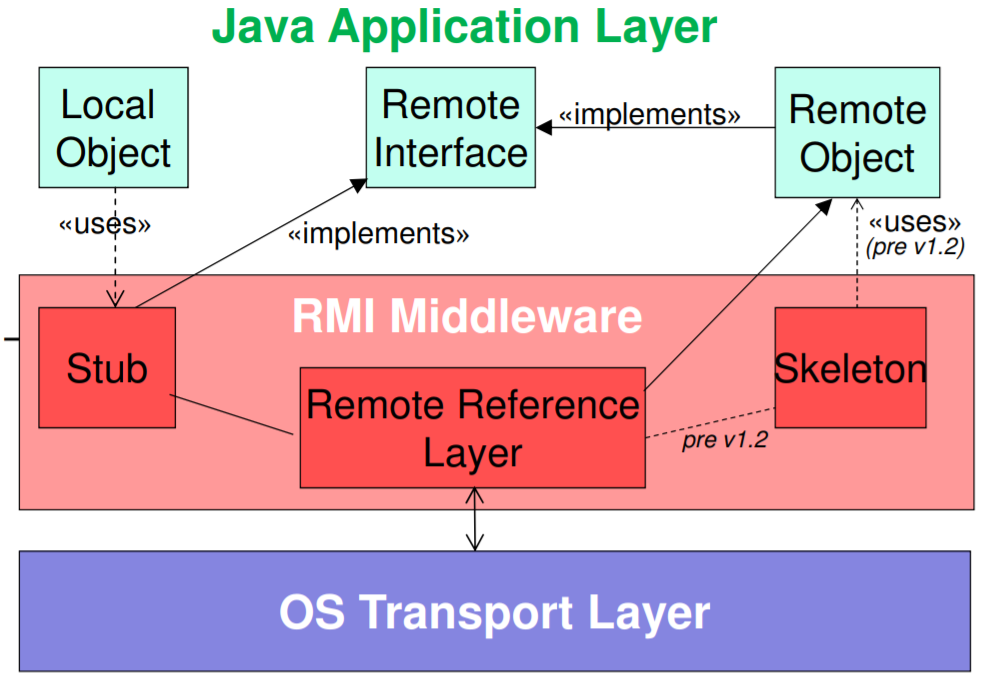
\includegraphics[scale=0.5]{Components.png}
\end{center}
Компонентите на RMI архитектурата са:
\begin{itemize}[noitemsep]
	\item \textbf{Транспортен слой} - Този слой свързва клиента и сървъра. Той управлява съществуващите връзки и също така създава нови такива.
	\item \textbf{Stub} - Това е представяне(прокси) на отдалечния обект, намиращ се на клиента. Използва се като конумикационна точка(интерфейс) на клиентската програма за методите на сървъра.
	\begin{itemize}[noitemsep]
		\item Генерират се отделно от \textbf{rmic} компилатора(преди Java SDK 6) или автоматично когато отдалеченият сървър бъде компилиран(след Java SDK 6).
		\item Поддържа вътрешна референция към отдалечения обект, който представлява.
		\item \enquote{Marshall}-ва аргументите на метода в серилизируема форма - това означава, че параметрите трябва да са серилизуреми по начало.
	\end{itemize}	  
	\item \textbf{Skeleton} - Той се намира в сървърното адресно простанство и служи като \textbf{server-side прокси} за отдалечения обект. 
	\begin{itemize}[noitemsep]
		\item RMI skeleton-a \enquote{unmarshalls} аргументите на методите
		\item Аргументите, които са отдалечени референции сами по себе си, водят до създаването на \textit{локален stub}
		\item Marshall-ва return стойността
		\item \textit{Skeleton-ите са deprecate-нати от RMI v1.2, като тяхната фунцкионалност се изпълнява от сървърния Remote Reference Layer}
	\end{itemize}
	\item RRL(Remote Reference Layer) - Този слой управлява референциите, направени от клиента към отдалечения обект.
\end{itemize}

\subsection{Отдалечен обект}
Отдалечен обект е такъв, който съществува на друга \textbf{виртуална} машина, която може да работи както на отдалечен компютър, така и на лоцален. Сървърите дефинират и инстанциират обекти, които клиентите могат да използват отдалечено чрез \textbf{отдалечени интерфейски}. Клиентите извикват методи върху отдалечените обекти. (след като са се свързали към тях чрез \textbf{отдалечени референции}). Аргументите и return стойностите на методите могат да са примитивни стойности или по-сложни, серилизируеми, обекти.
\begin{center}
	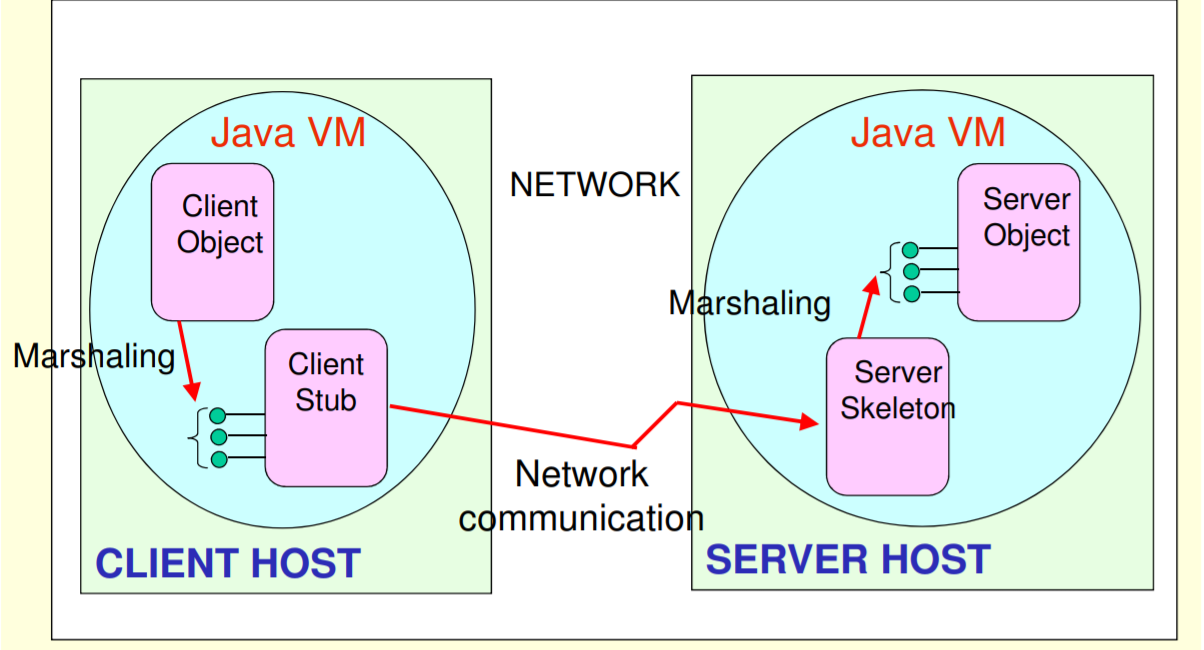
\includegraphics[scale=0.55]{RemoteObjects.png}
\end{center}

\textbf{Разработка на отдалечени обекти: }
\begin{enumerate}[noitemsep]
	\item Написваме source файловете:
	\begin{enumerate}[noitemsep]
		\item Дефинираме отдалечените методи в интерфейс
		\item Пишем сървърни/имплементационни класове
		\item Пишем клиентското приложение
	\end{enumerate}
	\item Компилираме и deploy-ваме клас-файловете
	\begin{enumerate}[noitemsep]
		\item Използваме \textbf{javac} да компилираме source файловете
		\item Използваме \textbf{rmic} да генерираме stub-ове/skeleton-и(преди SDK 6).
	\end{enumerate}
	\item Стартираме RMI регистъра, сървъра и клиента
\end{enumerate}

\section{Web услуги}
\definition Стандартизиран начин за интеграция на уеб-базирани приложения при използване на XML, SOAP, WSDL и UDDI отворените стандарти, основавайки се на интернет протокол. XML се използва за форматиране на данни, SOAP за тяхното трансфериране, WSDL - за описание на наличните услуги, а UDDI - за откриването им. 
\begin{center}
	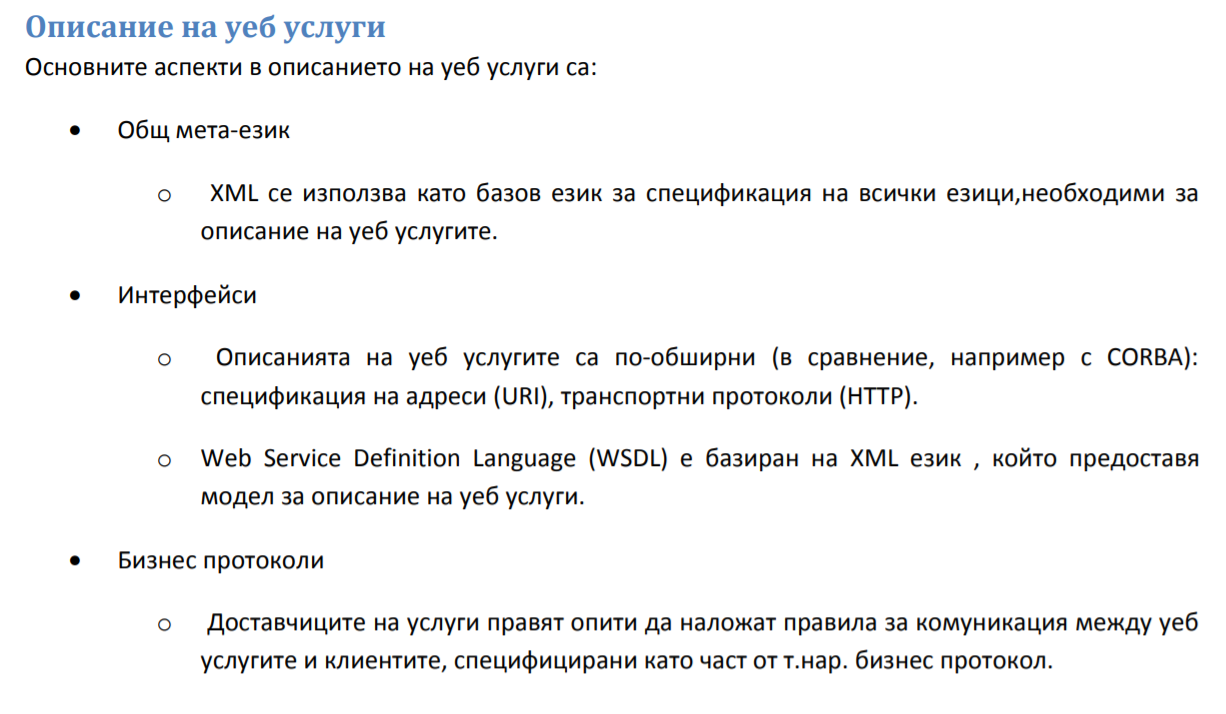
\includegraphics[scale=0.65]{WebServices1.png}
	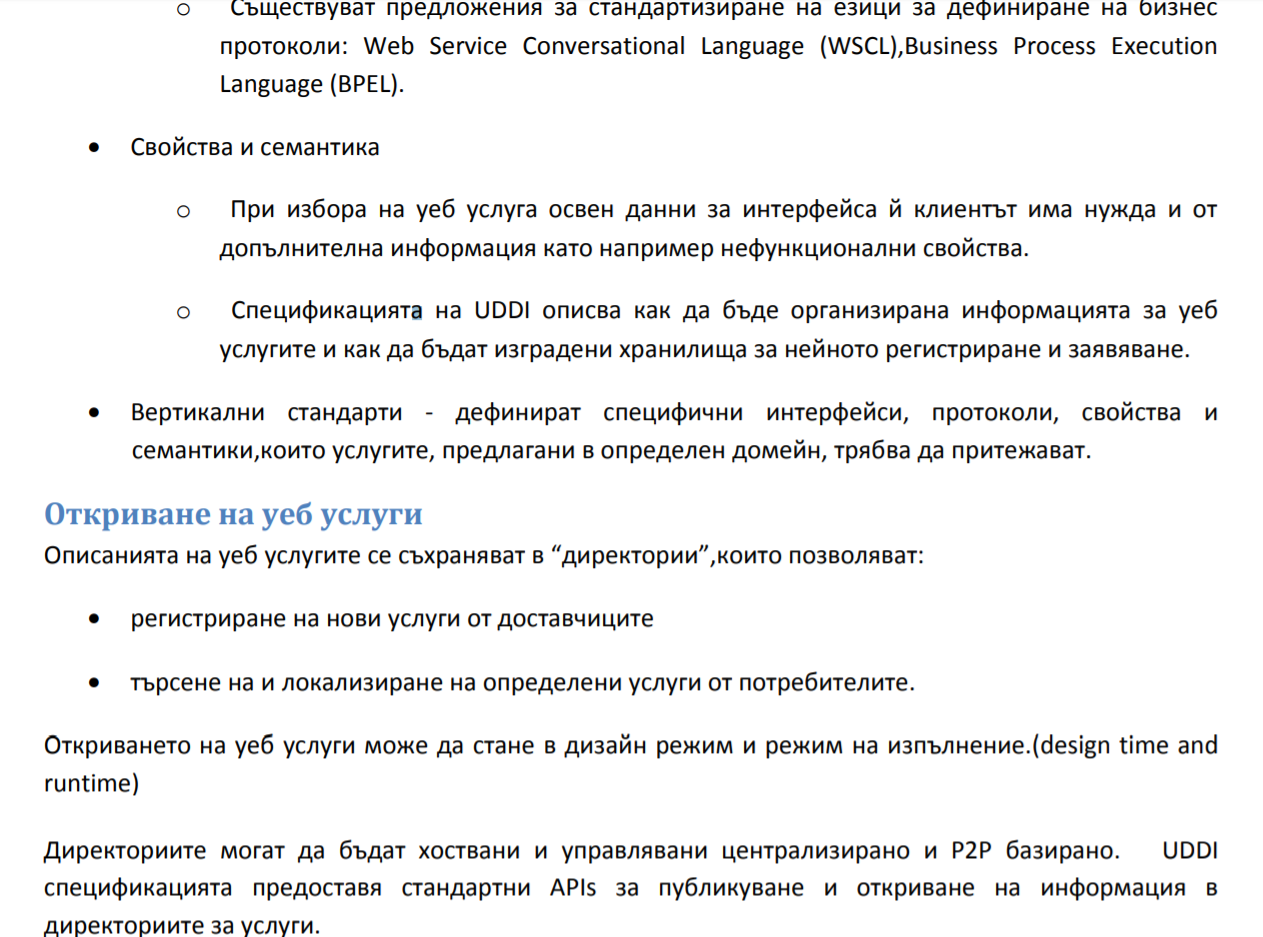
\includegraphics[scale=0.65]{WebServices2.png}
	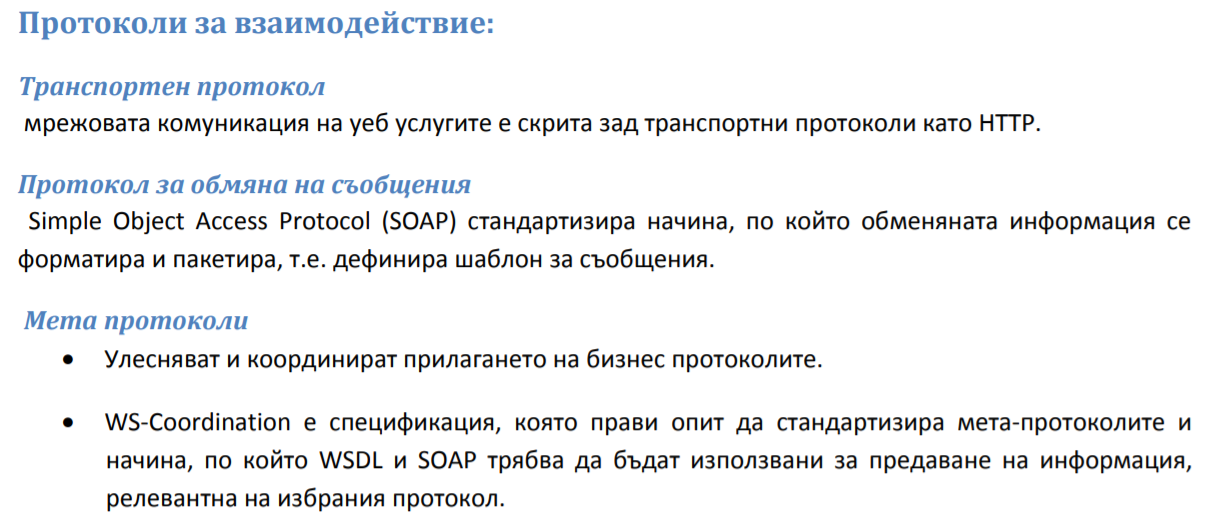
\includegraphics[scale=0.65]{WebServices3.png}
	
\includegraphics[scale=0.65]{WebServices4.png}
	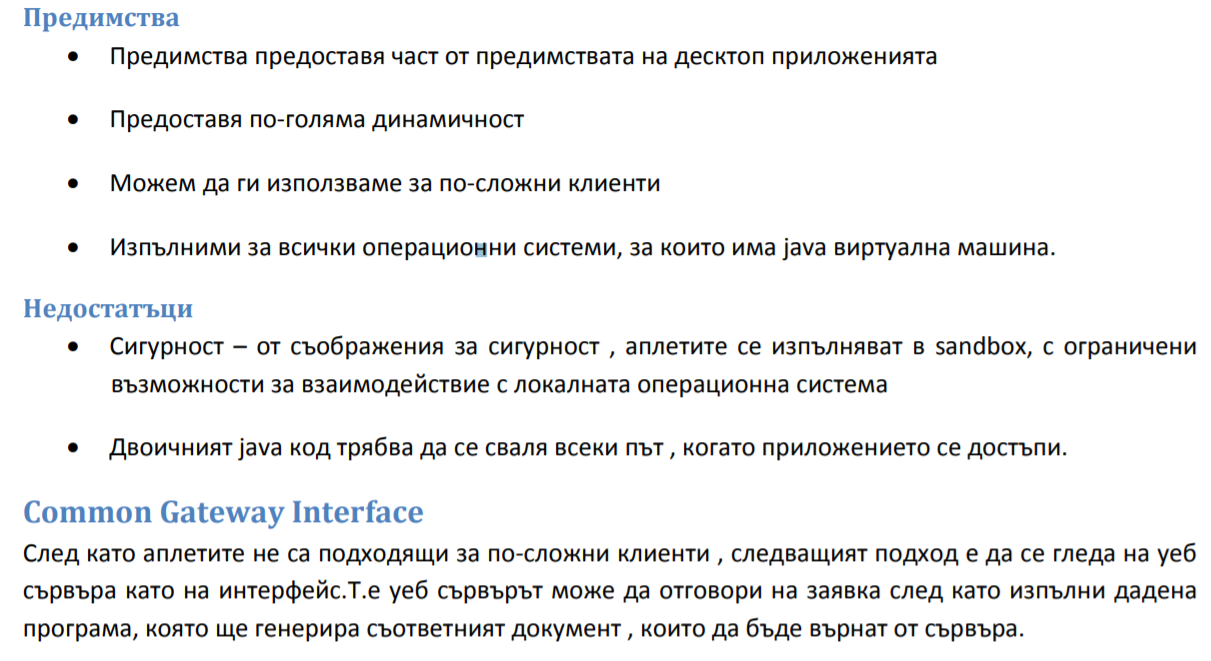
\includegraphics[scale=0.65]{WebServices5.png}
\end{center}
  
\end{document}






